\documentclass[12pt]{article}


\begin{document}
\subsubsection{Icosphère, c'est quoi ?}
L'Icosphère est une sphère construite par des triangles. La circonférence du cercle sera définie par le nombre de subdivisions effectuées. Pour être plus précis, la Figure \ref{fig:image_subdiv} montre l'icosphère selon le nombre de subdivisions effectuées.

\subsubsection{Comment la fabriquer ?}
Parmi toutes les classes de forme, la classe Icosphere prend le plus de temps à construire. 
Cette forme a été construite d'abord en definissant ses points en multipliant le point x, y et z dans un ordre particulier avec cette formule :
$$\frac{1+\sqrt{5}}{2}$$
Puis, on fabrique des triangles en utilisant ces points là et on les ajoute dans une liste de triangles.
Finallement, on affiche la liste de triangles.

\subsubsection{Subdivision.s}
La subdivision est un des paramètres du constructeur de la classe icosphère.
Théoriquement, on peut fabriquer la subdivision de l'icosphère en divisant chaque triangle de la subdivision d'avant en 4 triangles et ces nouveaux triangles vont rendre l'icosphère plus ronde.
L'image \ref{tab:image_subdiv} dessous montre la différence entre subdivision 1, 3 et 5 de l'icosphère.

\begin{figure}[ht]
  \begin{center}
    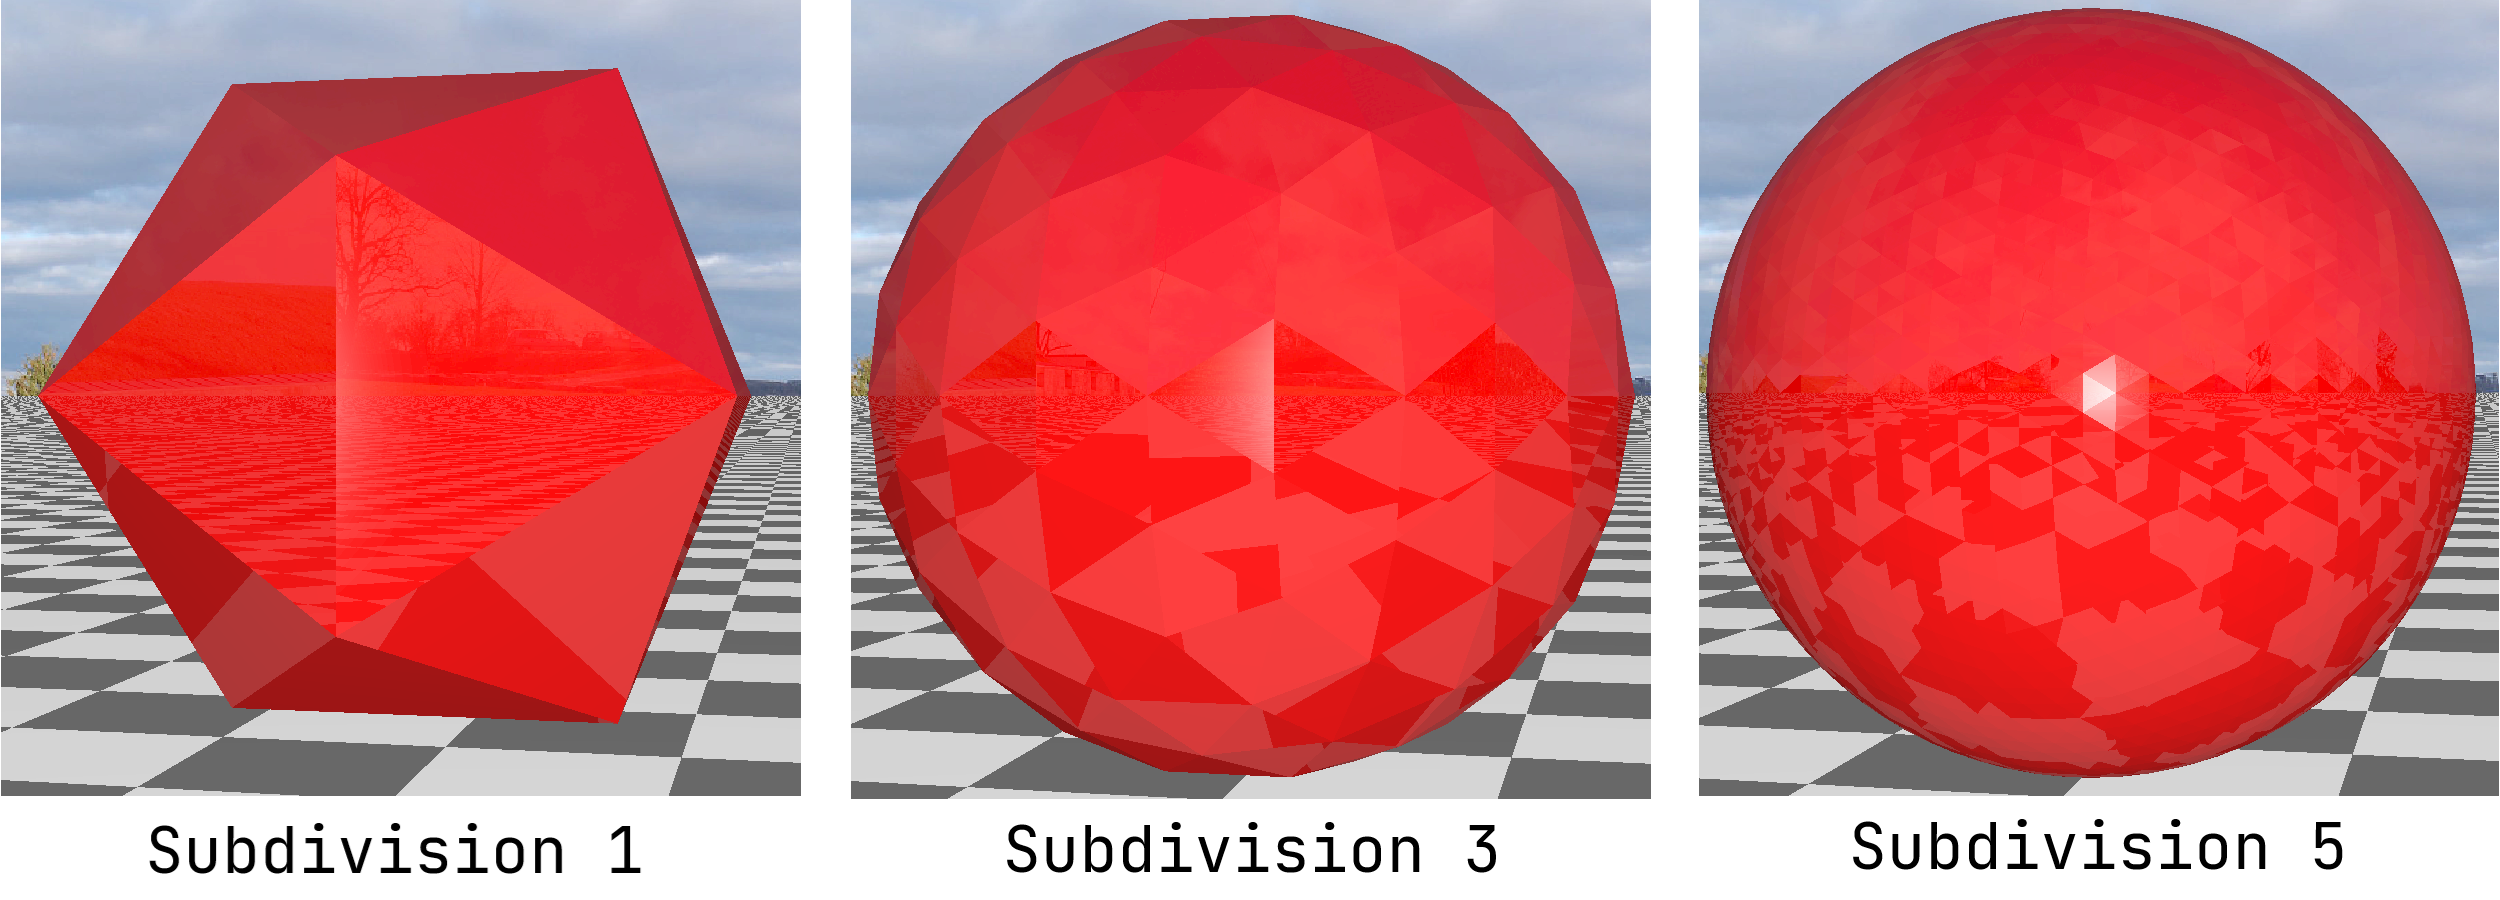
\includegraphics[width=0.7\textwidth]{./img/formes/subdivicosp.png} 
  \caption{Les subdivisions de l'icosphere qui forme une sphère composée par des triangles}
  \label{fig:image_subdiv}
\end{center}
\end{figure}
\FloatBarrier



\end{document}
